\documentclass[../main/main.tex]{subfiles}
% TODO: corriger avec éléments de rM2.

\raggedbottom

\makeatletter
\renewcommand{\@chapapp}{Architecture de la mati\`ere -- chapitre}
\makeatother

% \toggletrue{student}
% \HideSolutionstrue

\begin{document}
\setcounter{chapter}{2}

\chapter{Solides cristallins}

\setcounter{section}{3}
\section{Différents types de cristaux}
Les solides cristallins présentent des propriétés macroscopiques très
diversifiées. Par exemple, mécaniquement on distingue~:
\begin{itemize}
  \item la \textbf{dureté}~: résistance à la pénétration~;
  \item la \textbf{malléabilité}~: capacité à se déformer (par choc ou pression)
    sans rompre~;
  \item la \textbf{ductilité}~: capacité à être étiré sans casser.
\end{itemize}
On trouve également des propriétés électriques et chimiques (solubilité,
température de fusion).

On peut alors les regrouper par famille, selon leur structure microscopique dont
émergent les propriétés macro~: c'est l'objectif des paragraphes suivants.

\subsection{Cristaux métalliques}
\subsubsection{Description}
On peut décrire un cristal métallique comme une structure dans laquelle les
nœuds du réseau sont occupés par des \textbf{cations} (\ce{M+} ou \ce{M^{2+}},
perte d'un ou deux électrons de valence), et tous les électrons cédés sont
\textbf{délocalisés} sur l'ensemble du cristal. Cette délocalisation assure la
cohésion du cristal. Ainsi,
\begin{tprop}{Liaison métallique, heart}
  % \begin{hide}
  \cswitch{white}{
    \begin{center}
        La liaison métallique est \textbf{forte} ($E \approx
        \SI{100}{kJ.mol^{-1}}$) et \textbf{isotrope} (égale dans toutes les
        directions).
    \end{center}
  }
% \end{hide}
\end{tprop}

\begin{minipage}[t]{.45\linewidth}
  Conventionnellement, la limite entre métaux et non-métaux est définie comme
  sur la figure ci-contre, mais elle est relativement floue. Entre les deux, on
  a les semi-conducteurs (ou métalloïdes, ou semi-métaux), qui ont des
  propriétés métalliques peu marquées. De leur position dans le tableau
  périodique, on en conclue~:
\end{minipage}
\hfill
\begin{minipage}[t]{.45\linewidth}
  ~
  \vspace{-12pt}
  \begin{center}
    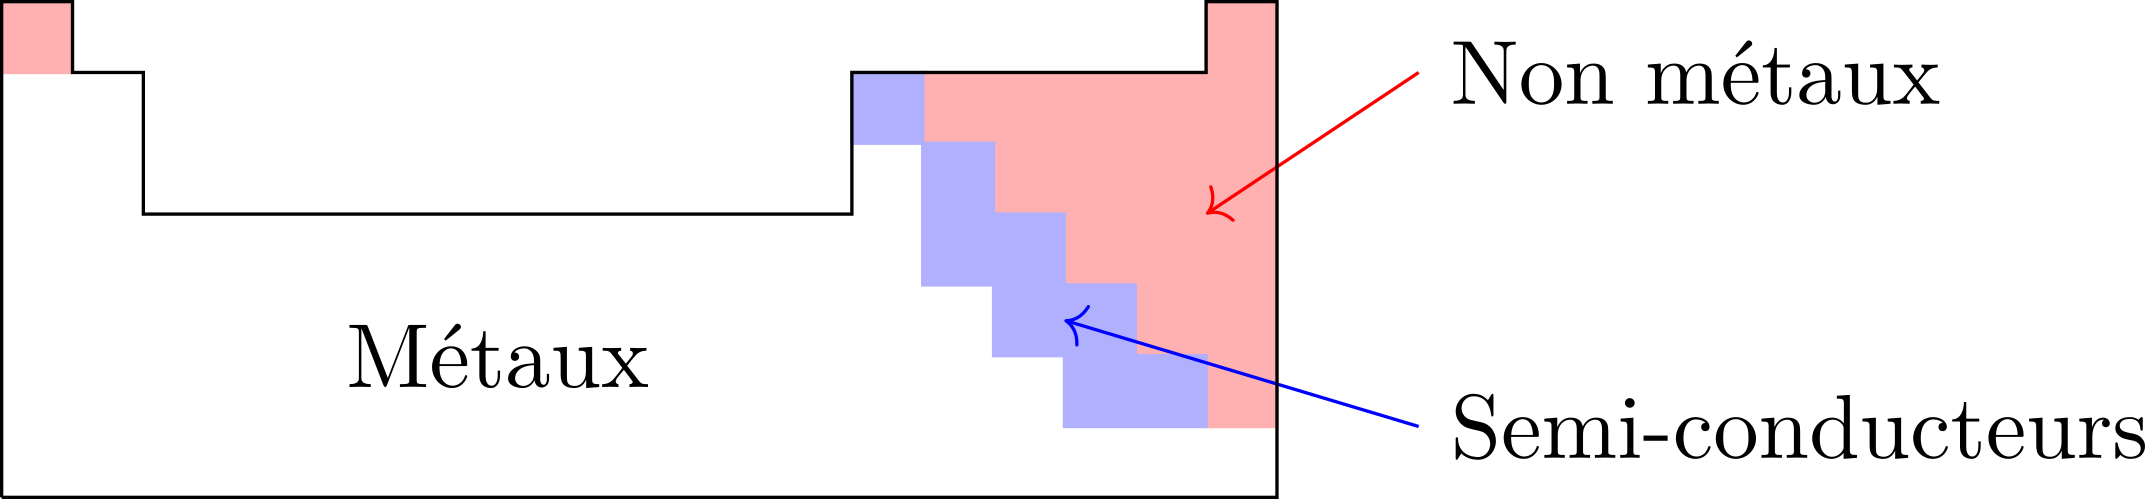
\includegraphics[scale=1]{metaux}
  \end{center}
\end{minipage}

\begin{tprop}{Électronégativité}
  \cswitch{white}{
    \begin{center}
      Un métal est un élément \textbf{peu électronégatif}.
    \end{center}
  }
\end{tprop}

À partir de ces propriétés macroscopiques, on peut expliquer les propriétés
macroscopiques~; voir Tableau~\ref{tab:ptemet}.
\begin{table}[ht]
  \renewcommand\arraystretch{1.6}
  \caption{Propriétés des cristaux métalliques}
  \label{tab:ptemet}
    \begin{tabularx}{\linewidth}{XcY}
      \toprule
      \multicolumn{1}{Y}{\textbf{Propriété microscopique}} & &
      \textbf{Propriété macroscopique}
      \\\midrule
      Liaison métallique forte & donc &
      \cswitch{white}{température de fusion élevée}
      \\\midrule
      Liaison isotrope donc atomes déplaçables & donc &
      \cswitch{white}{ductile et malléable}
      \\\midrule
      Électrons libres & donc &
      \cswitch{white}{conductivité électrique et thermique}
      \\\midrule
      Électrons facilement arrachés & donc &
      \cswitch{white}{métaux réducteurs}
      \\\bottomrule
    \end{tabularx}
\end{table}

\subsubsection{Alliages métalliques}
\begin{tdefi}{Définition, hand}
  \cswitch{white}{
    \begin{center}
        Un alliage est un cristal combinant un métal (dit \textit{de base}) avec
        un ou plusieurs autres éléments (dits \textit{d'alliage}), métalliques
        ou non.
    \end{center}}
\end{tdefi}

On dit aussi parfois qu'un alliage est une «~solution solide~»~: la base serait
le solvant, les autres les solutés. L'intérêt des alliages est de faire varier
les propriétés du matériau de base, notamment mécaniques et anti-corrosives. On
peut les réaliser de deux manières~:
\begin{enumerate}
  \item par \textbf{substitution}~: un atome se substitue à un autre en certains
    points du réseau~;
  \item par \textbf{insertion}~: des atomes s'insèrent dans les sites
    cristallographiques du réseau métallique.
\end{enumerate}

\begin{table}[ht]
  \renewcommand\arraystretch{1.3}
  \caption{Exemples d'alliages courants et utilisations}
  \label{tab:alliages}
  \begin{tabularx}{\linewidth}{YYYm{8cm}}
    \toprule
    \textbf{Nom de l'alliage} & \textbf{Élément principal} & \textbf{Éléments
    ajoutés} &
    \multicolumn{1}{>{\centering\arraybackslash}m{7cm}}{\textbf{Propriétés et
    utilisations}}
    \\\midrule
    Acier & Fer & Carbone 2\% & Plus dur que le fer. Très répandu, notamment en
    construction ou dans l'industrie automobile.
    \\
    Acier inoxydable & Fer & Carbone 2\%, chrome et nickel & Plus résistant à
    la corrosion que l'acier simple.
    \\
    Alliages d'aluminium & Aluminium & Cobalt, nickel, tantale & Alliages durs
    mais légers, utilisés notamment en aéronautique.
    \\
    Bronze & Cuivre > 60\% & Étain & Plus résistant que le cuivre à l'usure.
    Utilisé pour la décoration , la lutherie, la sculpture.
    \\
    Laiton & Cuivre > 60\% & Zinc & Plus dur et plus facile à usiner que le
    cuivre. Utilisé en horlogerie, serrurerie, robinetterie, lutherie.
    \\
    Or rose & Or & Cuivre 20\%, argent 5\% & Utilisé en joaillerie.
    \\
    Or blanc & Or & Argent & Utilisé en joaillerie, recouvert d'une couche de
    rhodium pour le rendre plus brillant.
    \\\bottomrule
  \end{tabularx}
\end{table}

\subsection{Cristaux ioniques}
\subsubsection{Description}
\begin{tdefi}{Cristal ionique, heart}
  \cswitch{white}{
    \begin{center}
        Un cristal ionique est un assemblage \textbf{électriquement neutre} de
        cations et d'anions.
    \end{center}
  }
\end{tdefi}
\begin{rexem}{Exercice}
  Déterminer la formule brute d'un cristal contenant les ions \ce{Fe3+} et
  \ce{O2-}.
  \tcblower
  \cswitch{white}{
    Pour avoir neutralité, pour chaque cation \ce{Fe3+} on doit avoir un nombre
    d'anion \ce{O2-} compensant la charge. En utilisant des nombres entiers, et
    les plus petits possibles, on trouve simplement
    \begin{center}
      \ce{Fe2O3}
    \end{center}
  }
\end{rexem}
La cohésion est alors assurée par les forces coulombiennes \textbf{entre} les
charges, à la fois d'attraction pour les charges opposées mais aussi de
répulsion pour les charges de même signe. Ainsi,
\begin{tprop}{Liaison ionique, heart}
  % \begin{hide}
  \cswitch{white}{
    \begin{center}
        La liaison des cristaux ioniques est \textbf{forte} ($E \gtrsim
        \SI{100}{kJ.mol^{-1}}$), \textbf{isotrope} mais \textbf{répulsive}.
    \end{center}
  }
% \end{hide}
\end{tprop}

Pour assurer leur stabilité, il est favorable qu'un maximum d'anions entoure de
manière compacte chaque cation. Ainsi, un cristal ionique est souvent décrit
comme un réseau d'anions où les cations occupent les sites cristallographiques
(ou inversement). Avec le modèle des sphères dures, on décrit le rayon des
entités par leur \textbf{rayon ionique}, et on considère le rayon des anions
plus grand que celui des cations (plus d'électrons en périphérie). On a donc
\begin{tprop}{Stabilité d'un cristal ionique de sphères dures}
  \cswitch{white}{
    \begin{center}
      Dans un cristal ionique, il y a contact cation/anion, mais pas anion/anion
      ou cation/cation, à la fois par répulsivité et par non-contact.
    \end{center}
  }
\end{tprop}

À partir de ces propriétés macroscopiques, on peut expliquer les propriétés
macroscopiques~:
\begin{table}[ht]
\renewcommand\arraystretch{1.6}
  \caption{Propriétés des cristaux ioniques}
  \label{tab:pteion}
    \begin{tabularx}{\linewidth}{XcY}
      \toprule
      \multicolumn{1}{Y}{\textbf{Propriété microscopique}} & &
      \textbf{Propriété macroscopique}
      \\\midrule
      Liaison ionique forte & donc &
      \cswitch{white}{température de fusion élevée}
      \\\midrule
      Liaison isotrope mais répulsive, ions fixes & donc &
      \cswitch{white}{indéformable}
      \\\midrule
      Électrons dans les liaisons & donc &
      \cswitch{white}{faible conductivité}
      \\\midrule
      Ions attirés par solvants polaires & donc &
      \cswitch{white}{forte solubilité avec
      solvants polaires}
      \\\bottomrule
    \end{tabularx}
\end{table}

\subsubsection{Exemples de cristaux ioniques}

\begin{wrapfigure}[3]{R}{.3\linewidth}
  \vspace*{-30pt}
  \centering
  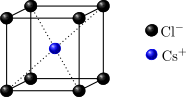
\includegraphics[width=.8\linewidth]{cscl}
\end{wrapfigure}
\paragraph*{La structure \ce{CsCl} (chlorure de césium)} est une structure
\textbf{cubique centrée}. En prenant le césium au centre et le chlore sur les
sommets, on a la géométrie suivante~:
\vspace{20pt}
\begin{itemize}[label=$\diamond$]
  \litem{Formule chimique}~:
    \cswitch{white}{on a $8\times1/8 = 1$ ion chlorure,
    et 1 ion césium dans la maille $\Ra$ \fbox{\ce{CsCl}}.}
    \vspace{20pt}
  \litem{Coordinence}~:
    \cswitch{white}{un cation a 8 anions plus proches voisins (contact) et 8
    cations, et inversement (on parle de structure 8-8).}
    \vspace{20pt}
  \litem{Condition géométrique}~:
  \begin{hide}
    contact anion/cation sur la \textbf{grande
    diagonale}, soit $a \sqrt{3} = 2r_{+} + 2r_{-}$, et
    \textbf{non-contact} sur une face soit $a > 2r_{-}$~:
    \begin{align*}
      \frac{2}{\sqrt{3}}r_{+} + \frac{2}{\sqrt{3}}r_{-} &> 2r_{-}
      \\\Lra
      r_{+} + r_{-} &> r_{-}\sqrt{3}
      \\\Lra
      \Aboxed{\frac{r_{+}}{r_{-}} &> \sqrt{3}-1 = \num{0.732}}
    \end{align*}
\end{hide}
    \vspace{20pt}
\end{itemize}

\begin{wrapfigure}[3]{R}{.3\linewidth}
  \vspace*{-30pt}
  \centering
  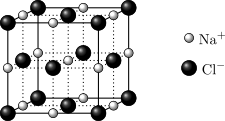
\includegraphics[width=.8\linewidth]{nacl}
\end{wrapfigure}
\paragraph*{La structure \ce{NaCl} (chlorure de sodium)} est une structure
\textbf{cubique faces centrées}. Les ions chlorure sont sur les nœuds, les ions
sodium sur les sites \textbf{octaédriques} (forme également un réseau CFC).

\begin{rexem}{Exercice}
  \begin{enumerate}
    \item Dénombrer les anions et cations dans la maille. En déduire la formule
      brute dans la maille.
    \item Déterminer la coordinence anions/cations.
    \item Montrer que la structure est stable~: il y a contact entre ions de
      charges opposées mais pas entre ions de même charge. On donne $r_{+} =
      \SI{95}{pm}$ et $r_{-} = \SI{181}{pm}$.
  \end{enumerate}
  \tcblower 
  \vspace{20pt}
  \cswitch{white}{
  \begin{enumerate}
    \litem{Formule chimique}~: $8\times1/8+6\times1/12=4$ ions chlorure, et
    $12\times1/4=4$ ions sodium dans la maille $\Ra$ \fbox{\ce{NaCl}}.
    \litem{Coordinence}~: un cation a 6 anions plus proches voisins (avec qui il
    est en contact), et 12 cations (et inversement) (on parle de structure 6-6).
    \litem{Condition géométrique}~: contact entre ions de charges opposées donne
    $a = 2r_{+} + 2r_{-}$. La condition de non-contact entre deux anions d'une
    face est $a \sqrt{2} > 4r_{-}$. Ainsi,
    \begin{align*}
      2r_{+}\sqrt{2} + 2r_{-}\sqrt{2} &> 4r_{-}
      \\\Lra
      r_{+} + r_{-} &> r_{-}\sqrt{2}
      \\\Lra
      \Aboxed{\frac{r_{+}}{r_{-}} &> \sqrt{2}-1 = \num{0.414}}
    \end{align*}
    Or, $r_{+}/r_{-} \approx \num{0.52}$~: la condition est bien respectée.
  \end{enumerate}
  }
  \vspace{20pt}
\end{rexem}

\vspace*{20pt}
\begin{wrapfigure}[3]{R}{.3\linewidth}
  \vspace*{-30pt}
  \centering
  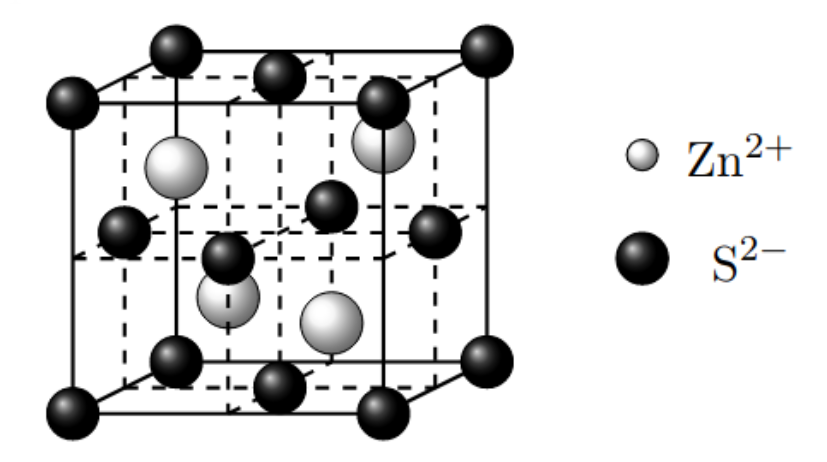
\includegraphics[width=.8\linewidth]{zns}
\end{wrapfigure}
\paragraph*{La structure \ce{ZnS} (sulfure de zinc)} est une structure
\textbf{cubique faces centrées}. Les ions sulfure sont sur les nœuds, les ions
zinc sur \textbf{un site tétraédrique sur deux}.
\vspace{20pt}
\begin{itemize}[label=$\diamond$]
  \litem{Formule chimique}~:
    \cswitch{white}{on a $8\times1/8 +6\times1/2 = 4$ ions sulfure,
    et 4 ions zinc dans la maille $\Ra$ \ce{Zn4S4} ou \fbox{\ce{CsCl}}.}
    \vspace{20pt}
  \litem{Coordinence}~:
    \cswitch{white}{un cation a 4 anions plus proches voisins (contact) et 12
    cations, et inversement (on parle de structure 4-4).}
    \vspace{20pt}
  \litem{Condition géométrique}~:
  \begin{hide}
    contact anion/cation sur la \textbf{grande
    diagonale d'un petit cube}, soit $a \sqrt{3}/2 = 2r_{+} + 2r_{-}$, et
    \textbf{non-contact} sur une face soit $a \sqrt{2} > 4r_{-}$~:
    \begin{align*}
      a \sqrt{2} &= 4 \sqrt{\frac{2}{3}}r_{+} + 4 \sqrt{\frac{2}{3}}r_{-}
      \\\Ra
      r_{-} &< r_{+}\sqrt{\frac{2}{3}} + r_{-}\sqrt{\frac{2}{3}}
      \\\Lra
      \Aboxed{\frac{r_{+}}{r_{-}} &> \sqrt{\frac{3}{2}}-1 = \num{0.225}}
    \end{align*}
\end{hide}
    \vspace{20pt}
\end{itemize}

\subsection{Cristaux covalents ou macrovalents}
\begin{tdefi}{Cristal covalent, heart}
  \cswitch{white}{
    \begin{center}
      Dans un cristal macrovalent, \textbf{tous} les atomes du cristal sont liés
      entre eux pas des liaisons covalentes.
    \end{center}
  }
\end{tdefi}
On trouvera ainsi principalement des éléments qui ne font peu d'ions, mais qui
font beaucoup de liaisons~: ceux avec une couche de valence environ à moitié
pleine, donc bloc d et la gauche du bloc p (carbone, silicium…).

\begin{tprop}{Liaison covalente, heart}
  % \begin{hide}
  \cswitch{white}{
    \begin{center}
        La liaison des cristaux covalents est \textbf{très forte} ($E \gtrsim
        \SI{300}{kJ.mol^{-1}}$) et \textbf{directionnelle}.
    \end{center}
  }
% \end{hide}
\end{tprop}

À partir de ces propriétés macroscopiques, on peut expliquer les propriétés
macroscopiques~; voir Tableau~\ref{tab:ptecov}.

\begin{rexem}{Exercice}
  \begin{wrapfigure}[4]{R}{.2\linewidth}
    \vspace*{-20pt}
    \centering
    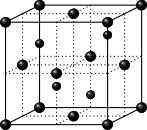
\includegraphics[width=.8\linewidth]{diamant}
  \end{wrapfigure}
  Le cas du carbone diamant est un cristal covalent, qui forme un réseau CFC
  avec la moitié des sites tétraédriques également occupés par des atomes de
  carbone.
  \begin{enumerate}
    \item Déterminer sa compacité.
    \item Déterminer sa masse volumique. On donne $a = \SI{356.7}{pm}$.
  \end{enumerate}
  \tcblower
  \vspace{20pt}
  \cswitch{white}{
    \begin{enumerate}
      \item Contact sur la grande diagonale d'un petit cube~: $a \sqrt{3}/2 =
        4r$. Or, on compte $4+6\times1/2+8\times1/8 = 8$ atomes par maille.
        Ainsi,
        \begin{align*}
          C &= \frac{NV_{\rm sph}}{V_{\rm m}}
          \\\Lra
            &= \frac{8\times \frac{4}{3}\pi r^3}{a^3}
          \\\Lra
            &= \frac{\frac{32}{3}\pi r^3}{\frac{512}{3 \sqrt{3}}r^3}
          \\\Lra
          \Aboxed{C &= \frac{\pi \sqrt{3}}{16} \approx \num{0.34}}
        \end{align*}
      \item La masse volumique, avec $M_{\ce{C}} = \SI{12}{g.mol^{-1}}$, est
        \[
          \boxed{
          \rho = \frac{NM}{\Nc_Aa^3} \approx \SI{3500}{kg.m ^{-1}}
          }
        \]
    \end{enumerate}
  }
  \vspace{20pt}
\end{rexem}

\begin{table}[ht]
\renewcommand\arraystretch{1.6}
  \caption{Propriétés des cristaux covalents}
  \label{tab:ptecov}
    \begin{tabularx}{\linewidth}{XcY}
      \toprule
      \multicolumn{1}{Y}{\textbf{Propriété microscopique}} & &
      \textbf{Propriété macroscopique}
      \\\midrule
      Liaison covalente très forte & donc &
      \cswitch{white}{température de fusion très
      élevée}
      \\\midrule
      Liaison directionnelle donc atomes fixes & donc &
      \cswitch{white}{indéformable}
      \\\midrule
      Électrons dans les liaisons & donc &
      \cswitch{white}{isolant électrique}
      \\\bottomrule
    \end{tabularx}
\end{table}

\subsection{Cristaux moléculaires}
\begin{tdefi}{Cristal moléculaire, heart}
  \cswitch{white}{
    \begin{center}
        Un cristal moléculaire est fait de \textbf{molécules} liées entre elles par
      des \textbf{liaisons de VdW} ou \textbf{liaisons hydrogènes}.
    \end{center}
  }
\end{tdefi}
Le modèle des sphères dures n'est pas toujours adapté dans ce cas, puisque leur
géométrie est souvent anisotrope~: les motifs sont \textbf{orientés} dans la
maille, de telle sorte qu'ils maximisent l'énergie de liaison.

\begin{tprop}{Liaison moléculaire, heart}
  % \begin{hide}
  \cswitch{white}{
    \begin{center}
        La liaison des cristaux moléculaires est \textbf{faible} ($E \lesssim
        \SI{10}{kJ.mol^{-1}}$ pour VdW, $\approx \SI{30}{kJ.mol^{-1}}$ pour les
        LH) et \textbf{directionnelle}.
    \end{center}
  }
% \end{hide}
\end{tprop}

À partir de ces propriétés macroscopiques, on peut expliquer les propriétés
macroscopiques~; voir Tableau~\ref{tab:ptemol}.
\begin{table}[ht]
\renewcommand\arraystretch{1.6}
  \caption{Propriétés des cristaux moléculaires}
  \label{tab:ptemol}
    \begin{tabularx}{\linewidth}{XcY}
      \toprule
      \multicolumn{1}{Y}{\textbf{Propriété microscopique}} & &
      \textbf{Propriété macroscopique}
      \\\midrule
      Liaisons VdW et LH faibles & donc &
      \cswitch{white}{température de fusion faible}
      \\\midrule
      Liaison directionnelle mais faible donc déplaçable & donc &
      \cswitch{white}{faible dureté}
      \\\midrule
      Électrons localisés dans les molécules & donc &
      \cswitch{white}{isolant électrique}
      \\\midrule
      Interactions intérieures similaires aux solvants & donc &
      \cswitch{white}{forte solubilité si solvant adapté}
      \\\bottomrule
    \end{tabularx}
\end{table}

\switch{}{\vspace*{-20pt}}
\section{Bilan}
\switch{}{\vspace*{-15pt}}
\begin{table}[h!]
  \renewcommand\arraystretch{2.0}
  \begin{center}
    \caption{Bilan des différents types de cristaux.}
    \label{tab:bilan}
    \begin{tabularx}{\linewidth}{XYYYY}
      \toprule
      &
      \textbf{Cristaux métalliques} &
      \textbf{Cristaux ioniques} &
      \textbf{Cristaux covalents} &
      \textbf{Cristaux moléculaires}
      \\\cmidrule(lr){2-5}
      \textbf{Exemples} &
      \ce{Fe}, \ce{Ca}, \ce{Zn} &
      \ce{NaCl}, \ce{KOH} &
      Diamant, \ce{Si}, \ce{Ge} &
      \ce{H2O}, \ce{I2}, \ce{CO2}
      \\\midrule
      \textbf{Type de liaisons} &
      \cswitch{white}{Métallique (é. délocalisés)} &
      \cswitch{white}{Ionique (entre + et -)} &
      \cswitch{white}{Covalente} &
      \cswitch{white}{VdW, LH}
      \\\midrule
      \textbf{Température de fusion} &
      \cswitch{white}{Élevée ($\approx \SI{e3}{\degreeCelsius}$) }&
      \cswitch{white}{Assez élevée ($\approx \SI{e2}{\degreeCelsius}$) }&
      \cswitch{white}{Élevée ($\approx \SI{e3}{\degreeCelsius}$) }&
      \cswitch{white}{Faible ($\lesssim \SI{100}{\degreeCelsius}$)}
      \\\midrule
      \textbf{Propriétés mécaniques} &
      \cswitch{white}{Dur, malléable, ductile }&
      \cswitch{white}{Dur mais cassant }&
      \cswitch{white}{Dur et peu malléable }&
      \cswitch{white}{Fragile}
      \\\midrule
      \textbf{Propriétés électriques} &
      \cswitch{white}{Conducteur} &
      \cswitch{white}{Isolant} &
      \cswitch{white}{Le plus souvent isolant }&
      \cswitch{white}{Isolant}
      \\\midrule
      \textbf{Propriétés de solubilisation} &
      \cswitch{white}{Insoluble} &
      \cswitch{white}{Très solubles dans polaires }&
      \cswitch{white}{Insoluble} &
      \cswitch{white}{Très solubles si adéquat}
      \\\bottomrule
    \end{tabularx}
  \end{center}
\end{table}

\end{document}
